\begin{figure}
\scriptsize{
\medskip
%%%%%%%%%%%%%%%%%%%%
$
\inferrule
{
}
{\jp \FH{\phi}{\skipstmt}{\phi}}
\;(\textsc{Skip})
$
\medskip
%%%%%%%%%%%%%%%%%%%%
$
\inferrule
{
P \not \in \dom(\refines)
}
{\jp \FH{\phi}{\assert{\locExpr}}{\phi}}
\;(\textsc{Assert1})
$
\medskip
%%%%%%%%%%%%%%%%%%%%
$
\inferrule
{
}
{\jp \FH{\phi \wedge \locExpr}{\assert{\locExpr}}{\phi}}
\;(\textsc{Assert2})
$
\medskip
%%%%%%%%%%%%%%%%%%%%
$
\inferrule
{
}
{\jp \FH{e}{\yield{e}}{e}}
\;(\textsc{Yield})
$
\medskip
%%%%%%%%%%%%%%%%%%%%
$
\inferrule
{
\actions(A) = (\rho, \alpha, m) \\ \phi_1 \Rightarrow \rho \\ \phi_1 \wedge \alpha \Rightarrow \phi_2
}
{\jp \FH{\phi_1}{\call{A}}{\phi_2}}
\;(\textsc{Atomic})
$
\medskip
%%%%%%%%%%%%%%%%%%%%
$
\inferrule
{
\specs(P) = (\phi, \tls, \psi) \\ H \neq \{\}
}
{\jp \FH{\phi}{\call{P}}{\psi}}
\;(\textsc{Proc1})
$
\medskip
%%%%%%%%%%%%%%%%%%%%
$
\inferrule
{
\specs(P) = (\phi, \tls, \psi) \\ P \in \dom(\refines) \\ \jp \FH{\phi}{\call{\refines(P)}}{\psi}
}
{\jp \FH{\phi}{\call{P}}{\psi}}
\;(\textsc{Proc2})
$
\medskip
%%%%%%%%%%%%%%%%%%%%
$
\inferrule
{
\specs(P) = (\phi, \tls, \psi)
}
{\jp \FH{\rho \wedge \phi}{\async{P'}}{\rho}}
\;(\textsc{Async})
$
\medskip
%%%%%%%%%%%%%%%%%%%%
$
\inferrule
{
\jp \FH{\phi_1 \wedge e}{s}{\phi_2}
}
{\jp \FH{\phi_1 \wedge e}{\ablock{e}{s}}{\phi_2}}
\;(\textsc{Ablock})
$
\medskip
%%%%%%%%%%%%%%%%%%%%
$
\inferrule
{
\jp \FH{\phi_1}{s_1}{\phi_2} \\ \jp \FH{\phi_2}{s_2}{\phi_3}
}
{\jp \FH{\phi_1}{s_1;s_2}{\phi_3}}
\;(\textsc{Seq})
$
\medskip
%%%%%%%%%%%%%%%%%%%%
$
\inferrule
{
\jp \FH{e \wedge \phi_1}{s_1}{\phi_2} \\ \jp \FH{\neg e \wedge \phi_1}{s_2}{\phi_2}
}
{\jp \FH{\phi_1}{\ite{\locExpr}{s_1}{s_2}}{\phi_2}}
\;(\textsc{Ite})
$
\medskip
%%%%%%%%%%%%%%%%%%%%
$
\inferrule
{
\jp \FH{e \wedge \locExpr}{s}{e}
}
{\jp \FH{e}{\while{e,m}{\locExpr}{s}}{e \wedge \neg \locExpr}}
\;(\textsc{While})
$
\medskip
%%%%%%%%%%%%%%%%%%%%

}
\caption{Sequential rules for partial correctness}
\label{fig:sequential-correctness}
\end{figure}

For each procedure $P$ such that $\mov(P) = \perp$, prove the following judgments:
\[
\jp \FH{\pre(P)}{\bodies(P)}{\post(P)}
\]

Let $\Yields(P)$ be the set of yield predicates in procedure $P$
and 
$\Yields = \bigcup_{P \in \ProcName \wedge \mov(P) = \perp}\Yields(P) \cup \{P \in \ProcName \mid \pre(P)\} \cup \{P \in \ProcName \mid \post(P)\}$.
Let $\Ablocks(P)$ be the set of atomic blocks in procedure $P$.
Given a predicate $\phi$, let $\hat{\phi}$ represent $\phi$ with all thread-local and local 
variables substituted with fresh constants.

For each predicate $\phi \in \Yields$
and for each atomic block $\ablock{e}{s} \in \bigcup_{P \in \ProcName \wedge \mov(P) = \perp} \Ablocks(P)$, prove the following judgment:
\[
\jp \FH{\hat{\phi} \wedge e}{s}{\hat{\phi}}
\]

For each predicate $\phi \in \Yields$ and for each $P$ such that $\mov(P) \neq \perp$, prove the following judgment:
\[
\hat{\phi} \wedge \pre(P) \wedge \act(P) \Rightarrow \hat{\phi}
\]

\begin{figure}
\scriptsize{
\medskip
%%%%%%%%%%%%%%%%%%%%
$
\inferrule
{
}
{P \vdash \skipstmt : \epsilon}
\;(\textsc{Skip})
$
\medskip
%%%%%%%%%%%%%%%%%%%%
$
\inferrule
{
}
{P \vdash \assert{\locExpr} : \epsilon}
\;(\textsc{Assert})
$
\medskip
%%%%%%%%%%%%%%%%%%%%
$
\inferrule
{
}
{P \vdash \yield{e} : \epsilon}
\;(\textsc{Yield})
$
\medskip
%%%%%%%%%%%%%%%%%%%%
$
\inferrule
{
\mov(P') \neq \perp \\ \act(P') \Rightarrow \havoc{H}
}
{P \vdash \call{P'} : \epsilon}
\;(\textsc{Call-Loop})
$
\medskip
%%%%%%%%%%%%%%%%%%%%
$
\inferrule
{
\mov(P') \neq \perp \\ \act(P') \Rightarrow \act{P}
}
{P \vdash \ablock{e}{s} : A}
\;(\textsc{Call-Action})
$
\medskip
%%%%%%%%%%%%%%%%%%%%
$
\inferrule
{
\mov(P') \neq \perp \\ \act(P') \Rightarrow \havoc{H}
}
{P \vdash \async{P'} : \epsilon}
\;(\textsc{Async})
$
\medskip
%%%%%%%%%%%%%%%%%%%%
$
\inferrule
{
\jp \FH{e}{s}{\havoc{H \cup L}}
}
{P \vdash \ablock{e}{s} : \epsilon}
\;(\textsc{Ablock-Loop})
$
\medskip
%%%%%%%%%%%%%%%%%%%%
$
\inferrule
{
\jp \FH{e}{s}{\act(P)}
}
{P \vdash \ablock{e}{s} : A}
\;(\textsc{Ablock-Action})
$
\medskip
%%%%%%%%%%%%%%%%%%%%
$
\inferrule
{
P \vdash s_1 : \re_1 \\ P \vdash s_2 : \re_2
}
{P \vdash s_1;s_2 : \re_1\cdot\re_2}
\;(\textsc{Seq})
$
\medskip
%%%%%%%%%%%%%%%%%%%%
$
\inferrule
{
P \vdash s_1 : \re_1 \\ P \vdash s_2 : \re_2
}
{P \vdash \ite{\locExpr}{s_1}{s_2} : \re_1+\re_2}
\;(\textsc{Ite})
$
\medskip
%%%%%%%%%%%%%%%%%%%%
$
\inferrule
{
P \vdash s : \re
}
{P \vdash \while{e,m}{\locExpr}{s} : \re^*}
\;(\textsc{While})
$
\medskip
%%%%%%%%%%%%%%%%%%%%

}
\caption{Refinement rules}
\label{fig:refinement}
\end{figure}


\begin{figure}
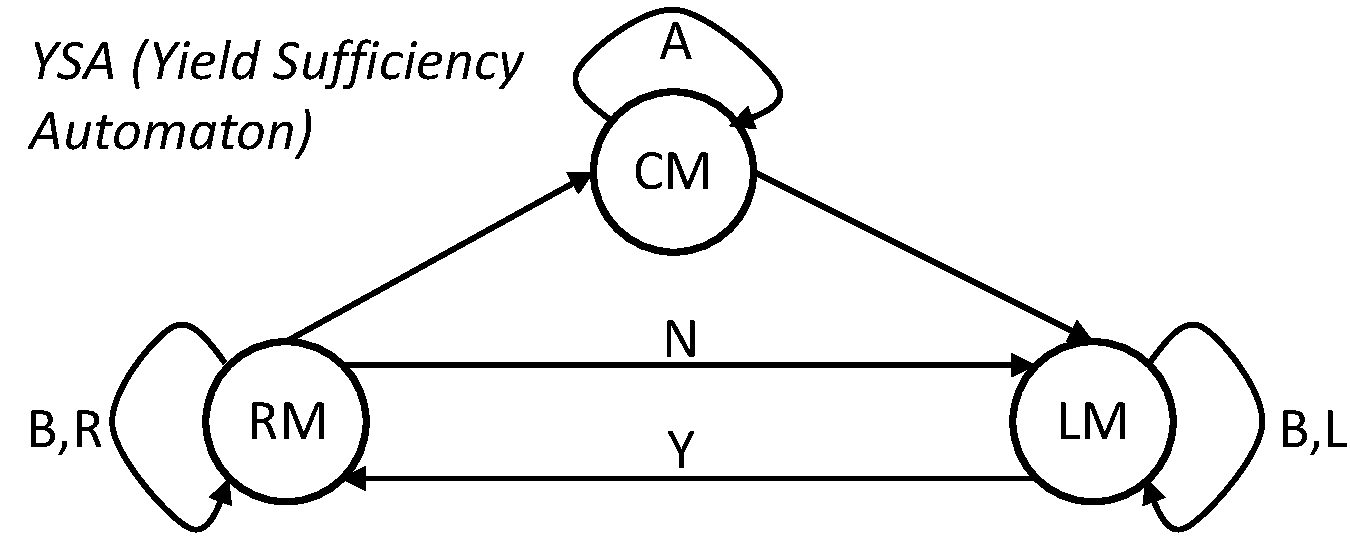
\includegraphics[scale=0.35]{YieldTypeCheckingAutomaton.pdf}
\caption{Specification for yield sufficiency}
\label{fig:YieldTypeCheckingAutomaton}
\end{figure}

\begin{figure}
\scriptsize{
\medskip
%%%%%%%%%%%%%%%%%%%%
$
\inferrule
{
}
{P \vdash \skipstmt : x \leadsto x}
\;(\textsc{Skip})
$
\medskip
%%%%%%%%%%%%%%%%%%%%
$
\inferrule
{
}
{P \vdash \assert{\locExpr} : x \leadsto x}
\;(\textsc{Assert})
$
\medskip
%%%%%%%%%%%%%%%%%%%%
$
\inferrule
{
}
{P \vdash \yield{e} : x \leadsto \RM}
\;(\textsc{Yield})
$
\medskip
%%%%%%%%%%%%%%%%%%%%
$
\inferrule
{
\mov(P') = B
}
{P \vdash \call{P'} : x \leadsto x}
\;(\textsc{CallBothMover})
$
\medskip
%%%%%%%%%%%%%%%%%%%%
$
\inferrule
{
\mov(P') = R
}
{P \vdash \call{P'} : \RM \leadsto \RM}
\;(\textsc{CallRightMover})
$
\medskip
%%%%%%%%%%%%%%%%%%%%
$
\inferrule
{
\mov(P') = L
}
{P \vdash \call{P'} : x \leadsto \LM}
\;(\textsc{CallLeftMover})
$
\medskip
%%%%%%%%%%%%%%%%%%%%
$
\inferrule
{
\mov(P') = N
}
{P \vdash \call{P'} : \RM \leadsto \LM}
\;(\textsc{CallYield})
$
\medskip
%%%%%%%%%%%%%%%%%%%%
$
\inferrule
{
\mov(P') = \perp
}
{P \vdash \call{P'} : x \leadsto \RM}
\;(\textsc{CallYield})
$
\medskip
%%%%%%%%%%%%%%%%%%%%
$
\inferrule
{
}
{P \vdash \async{P'} : x \leadsto \LM}
\;(\textsc{Async})
$
\medskip
%%%%%%%%%%%%%%%%%%%%
$
\inferrule
{
x \in \{\RM,\CM\}
}
{P \vdash \ablock{e}{s} : x \leadsto \CM}
\;(\textsc{Ablock})
$
\medskip
%%%%%%%%%%%%%%%%%%%%
$
\inferrule
{
P \vdash s_1 : x \leadsto y \\ P \vdash s_2 : y \leadsto z
}
{P \vdash s_1;s_2 : x \leadsto z}
\;(\textsc{Seq})
$
\medskip
%%%%%%%%%%%%%%%%%%%%
$
\inferrule
{
P \vdash s_1 : x \leadsto y \\ P \vdash s_2 : x \leadsto y
}
{P \vdash \ite{\locExpr}{s_1}{s_2} : x \leadsto y}
\;(\textsc{Ite})
$
\medskip
%%%%%%%%%%%%%%%%%%%%
$
\inferrule
{
P \vdash s : x \leadsto x
}
{P \vdash \while{e,m}{\locExpr}{s} : x \leadsto x}
\;(\textsc{While})
$
\medskip
%%%%%%%%%%%%%%%%%%%%

}
\caption{Yield sufficiency rules}
\label{fig:yield-sufficiency}
\end{figure}

\subsection{Responsiveness}

\begin{figure}
\scriptsize{
\medskip
%%%%%%%%%%%%%%%%%%%%
$
\inferrule
{
}
{\jr \FH{\phi}{\skipstmt}{\phi}}
\;(\textsc{Skip})
$
\medskip
%%%%%%%%%%%%%%%%%%%%
$
\inferrule
{
}
{\jr \FH{\phi}{\assert{\locExpr}}{\false}}
\;(\textsc{Assert})
$
\medskip
%%%%%%%%%%%%%%%%%%%%
$
\inferrule
{
}
{\jr \FH{\phi}{\yield{e}}{\false}}
\;(\textsc{Yield})
$
\medskip
%%%%%%%%%%%%%%%%%%%%
$
\inferrule
{
\phi_1 \wedge \specs(A) \Rightarrow \phi_2
}
{\jr \FH{\phi_1}{\call{A}}{\phi_2}}
\;(\textsc{Atomic})
$
\medskip
%%%%%%%%%%%%%%%%%%%%
$
\inferrule
{
\mov(P') = \perp
}
{\jr \FH{\phi}{\call{P'}}{\false}}
\;(\textsc{Call1})
$
\medskip
%%%%%%%%%%%%%%%%%%%%
$
\inferrule
{
\mov(P') \neq \perp \\ \phi_1 \wedge \act(P') \Rightarrow \phi_2
}
{\jr \FH{\phi_1}{\call{P'}}{\phi_2}}
\;(\textsc{Call2})
$
\medskip
%%%%%%%%%%%%%%%%%%%%
$
\inferrule
{
}
{\jr \FH{\phi}{\async{P'}}{\phi}}
\;(\textsc{Async})
$
\medskip
%%%%%%%%%%%%%%%%%%%%
$
\inferrule
{
\jr \FH{\phi_1 \wedge e}{s}{\phi_2}
}
{\jr \FH{\phi_1 \wedge e}{\ablock{e}{s}}{\phi_2}}
\;(\textsc{Ablock})
$
\medskip
%%%%%%%%%%%%%%%%%%%%
$
\inferrule
{
\jr \FH{\phi_1}{s_1}{\phi_2} \\ \jr \FH{\phi_2}{s_2}{\phi_3}
}
{\jr \FH{\phi_1}{s_1;s_2}{\phi_3}}
\;(\textsc{Seq})
$
\medskip
%%%%%%%%%%%%%%%%%%%%
$
\inferrule
{
\jr \FH{e \wedge \phi_1}{s_1}{\phi_2} \\ \jr \FH{\neg e \wedge \phi_1}{s_2}{\phi_2}
}
{\jr \FH{\phi_1}{\ite{\locExpr}{s_1}{s_2}}{\phi_2}}
\;(\textsc{Ite})
$
\medskip
%%%%%%%%%%%%%%%%%%%%
$
\inferrule
{
\jr \FH{e \wedge \locExpr}{s}{e \wedge m' < m} \\ e \wedge \locExpr \Rightarrow m \geq 0
}
{\jr \FH{e}{\while{e,m}{\locExpr}{s}}{e \wedge \neg \locExpr}}
\;(\textsc{While})
$
\medskip
%%%%%%%%%%%%%%%%%%%%

}
\caption{Sequential rules for responsiveness}
\label{fig:termination-correctness}
\end{figure}
